\documentclass[twoside]{article}

% Template: AISTATS 2026 (current). Switch to icml2026.sty for ICML submission.
\usepackage{aistats2026}
\usepackage{lmodern}
\usepackage{microtype}
\usepackage{graphicx}
\usepackage{subcaption}
\usepackage{booktabs}
\usepackage{etoolbox}
\PassOptionsToPackage{hyphens}{url}
\usepackage{hyperref}
\hypersetup{breaklinks=true}

\usepackage{amsmath}
\usepackage{amssymb}
\usepackage{mathtools}
\usepackage{amsthm}
\usepackage[capitalize,noabbrev]{cleveref}

\newtheorem{proposition}{Proposition}

\raggedbottom
% Switch to non-linked breakable URLs inside the bibliography so url.sty can
% insert break opportunities at '/' and '-', avoiding column overflow.
% \url is a robust command; its actual implementation lives in the internal
% \csname url \endcsname token. We redirect that token to url.sty's raw \Url
% formatter, which inserts break opportunities without a PDF link annotation.
\AtBeginEnvironment{thebibliography}{%
  \raggedright\sloppy
  \expandafter\let\csname url \endcsname\Url
}
\setlength{\emergencystretch}{3em}

\newcommand{\method}{CS-DSOS}
\newcommand{\sourceDist}{\mathcal{S}}
\newcommand{\targetDist}{\mathcal{T}}
\newcommand{\overlap}{\mathcal{O}}

\begin{document}

\twocolumn[

\aistatstitle{Testing Harmful Shift on Common Support}

\aistatsauthor{ Anonymous Authors }

\aistatsaddress{ Anonymous Institution }

]

\begin{abstract}
Testing for harmful shift asks whether the target worsened. When source and target samples have weak overlap, standard tests can reject even when the target did not worsen on the common support, the region where both samples have substantial overlap. Equal weighting lets observations from weak-overlap regions contaminate the comparison. We introduce CS-DSOS, a family of stabilized density-ratio weights from a domain classifier that restrict the comparison to the common support by downweighting observations unlikely to appear in the other environment. On HELOC, the FICO credit-risk benchmark, all three standard modes reject at the permutation minimum $p = 0.002$; the doubly weighted test does not reject ($p = 0.376$), revealing that the standard rejection was driven by applicant profiles from weak-overlap regions rather than model deterioration. Across synthetic and real-world tasks, the doubly weighted test reduces false alarms from weak overlap without attenuating power for genuine harmful change.

\end{abstract}

\section{Introduction}\label{sec:introduction}
Standard tests for harmful shift cannot separate two questions: did the model
get worse, or did the population just change? When deployment and training
samples barely overlap, observations from regions where only one side has data
can drive rejection even when the target did not worsen on the common support,
the region where both samples have substantial overlap.

The HELOC credit-risk dataset illustrates this failure mode. A model trained on
lower-risk applicants (external risk estimate above 63) is deployed on
higher-risk applicants (estimate at or below 63)~\cite{Gardner_2023}. Mean
predicted default risk rises from 44\% to 81\%---a large shift that could
indicate model harm or merely context change. All three standard
modes---unweighted, source-weighted, and target-weighted---reject at the
permutation minimum $p = 0.002$. Most of each population lies outside the common
support. The doubly weighted test, which adjusts both sides, does not reject
($p = 0.376$). The original rejection was driven by context change---applicant
profiles from weak-overlap regions that produce higher predicted risk---rather
than model harm on comparable cases. One-sided corrections still reject because
each corrects only one side (Figure~\ref{fig:heloc-motivating}).

\begin{figure}[t]
	\centering
	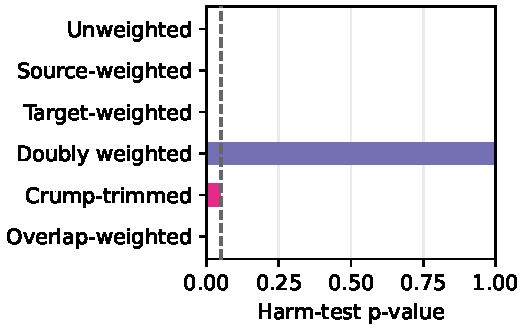
\includegraphics[width=0.92\linewidth]{figures/heloc_motivating_example_plot.pdf}
	\caption{HELOC credit-risk motivating example. Horizontal bar chart with
	weighting modes on the y-axis and harm-test $p$-value on the x-axis. The
	dashed line marks the 0.05 decision threshold. All three standard modes
	(unweighted, source-weighted, target-weighted) reject; the doubly weighted
	test does not. Effective sample sizes after reweighting to common support:
	source 401 of 1,536; target 803 of 2,776. The non-rejection indicates
	that comparable applicants receive similar predictions on common
	support.}
	\label{fig:heloc-motivating}
\end{figure}

The same ambiguity appears in the National Supported Work (NSW) employment
experiment~\cite{LaLonde_1986}, where the unweighted test fails to reject
($p = 0.350$)---a non-rejection that common-support restriction does not
reverse, illustrating that contamination can mask harm as readily as it invents
it. Together, HELOC and NSW demonstrate that weak-overlap contamination can
both invent harm and hide it.

Our starting point is D-SOS~\cite{pmlr-v180-kamulete22a}, a non-parametric
permutation test for one-sided harmful shift that compares the full observed
populations with uniform weights, allowing observations from low-overlap
regions to contaminate the comparison.\footnote{D-SOS calls the user-defined
quantity outlier scores; we use severity score to emphasize that larger
values mean worse behavior.}

We insert a weighting step that restricts the comparison to common support.
Stabilized density-ratio weights from a domain
classifier~\cite{Bickel_2007,Yamada_2013} downweight observations unlikely
to appear in the other environment---an approach the causal inference
literature developed for treatment-effect comparisons~\cite{Crump_2009,
Morgan_2015}. These weights apply to any two-sample test that accepts
per-observation weights. A single parameter $\lambda \in [0, 1]$ controls
the tradeoff between strict common-support restriction and the unweighted
comparison.

We call the resulting method CS-DSOS. The doubly weighted mode, which corrects
both source and target simultaneously, targets the common support and resolves
two-sided overlap contamination. Source-weighted and target-weighted modes serve
as asymmetric diagnostics for one-sided mismatch.

Our contributions are:
\begin{itemize}
\item CS-DSOS, a family of stabilized density-ratio weights that restrict
  harmful-shift testing to the common support. The doubly weighted mode
  corrects both source and target simultaneously and resolves two-sided
  overlap contamination, with source-weighted and target-weighted modes as
  asymmetric diagnostics for one-sided mismatch.
\item Evidence that the doubly weighted test removes false alarms from
  low-overlap contamination without attenuating power for genuine harmful
  change on the common support, across synthetic and real-world tasks.
\end{itemize}


\section{Related Work}
Most monitoring tools detect any distribution change irrespective of direction. Restricting the comparison to common support---the question closest to this paper---draws on three weighting traditions: hard threshold trimming, continuous propensity-score weighting, and density-ratio stabilization.

\paragraph{Overlap trimming and weighting in causal inference.}
Restricting comparisons to common support is familiar from causal inference, where treatment and control groups rarely share full covariate support. Three approaches define the space of options.

Crump et al.~\cite{Crump_2009} formalized \emph{overlap trimming}: discard observations where the propensity score $e(x)$ falls below a threshold $\alpha$ or above $1-\alpha$, then estimate the treatment effect on the remainder. The hard threshold discards data and introduces sensitivity to $\alpha$.

Li et al.~\cite{Li_2018_balancing,Li_2019} developed \emph{overlap weights}, assigning continuous weight $w(x) = e(x)(1-e(x))$ to each observation. This targets the subpopulation with most treatment equipoise. Unlike Crump trimming, the weight approaches zero smoothly rather than by cutoff. Overlap weights are bounded ($\max = 0.25$), symmetric, and treat both groups identically.

Morgan and Winship~\cite{Morgan_2015} provide the counterfactual framework that connects overlap to estimand identification.

\paragraph{Density-ratio weighting for covariate shift.}
A separate line of work uses the \emph{density ratio} $r(x) = p_{\mathrm{tgt}}(x) / p_{\mathrm{src}}(x)$ rather than the propensity score. Bickel et al.~\cite{Bickel_2007} showed that a classifier distinguishing source from target yields covariate-shift correction weights via Bayes' theorem: $r(x) = \frac{p}{1-p} \cdot \frac{n_s}{n_t}$.

Density-ratio and overlap weights use the same domain probabilities but transform them differently: RIW incorporates the prior ratio from group sizes and produces weights monotonic in the relative density of the two groups rather than symmetric around $p=0.5$. The raw ratio is unbounded, so practitioners apply stabilization. Yamada et al.~\cite{Yamada_2013} introduced relative importance weighting (RIW), which blends the density ratio toward uniform via a parameter $\lambda \in [0,1]$. Kanamori et al.~\cite{Kanamori_2012} and Sugiyama et al.~\cite{Sugiyama_2012} developed related unconstrained least-squares approaches.

The key distinction is that RIW targets the \emph{density ratio} while overlap weights target the \emph{propensity score variance}. Both produce continuous, bounded weights that downweight extremes, but the weight shape diverges under asymmetric overlap---precisely where overlap weights fail and the doubly weighted RIW correction succeeds (Section~\ref{sec:calibration}, Table~\ref{tab:weighting-benchmarks}).

Segovia-Mart{\'\i}n et al.~\cite{SegoviaMartin_2023} found that estimating density ratios for both source and target---a ``doubly weighted'' correction---improves finite-sample behavior over a single correction in the any-change two-sample testing setting.

\paragraph{Harmful-shift detection.}
The closest non-sequential directional test is D-SOS~\cite{pmlr-v180-kamulete22a}, which formalized the one-sided harmful-shift objective on the full observed population. Our contribution inserts a weighting step that restricts the comparison to the common support.

\paragraph{Risk tracking and sequential monitoring.}
Podkopaev and Ramdas~\cite{Podkopaev_Ramdas_2022} formalized harmful shift as a risk-function increase with sequential tests. Nguy{\~e}n et al.~\cite{Nguyen_D3M_2025}, Amoukou et al.~\cite{Amoukou_2024}, Prinster et al.~\cite{Prinster_2025}, and Ginsberg et al.~\cite{Ginsberg_2023} extended risk tracking to label-free, conformal, and learning-based settings. These methods operate sequentially or require a trained harm proxy---neither condition applies to our setting.

\paragraph{Conditional distribution testing.}
Cobb and Van Looveren~\cite{pmlr-v162-cobb22a} proposed context-aware drift detection by comparing predictor residuals. Hu and Lei~\cite{Hu_2024} developed a conformal conditional distribution test. Xu et al.~\cite{Xu_2024_crt} corrected the conditional randomization test using importance weights. These methods ask whether the \emph{relationship} between features and outcome changed---complementary to whether the outcome distribution itself worsened.

\paragraph{Common-support tests.}
Gagnon-Bartsch and Shem-Tov~\cite{GagnonBartsch_2019} introduced the Classification Permutation Test, which tests whether treated and control groups share common support by combining a classifier with permutation inference. Their test statistic is classifier accuracy rather than weighted scores, and the null is exchangeability rather than directional harm.


\section{Method}\label{sec:method}
The core change is to the comparison weights, not to the one-sided test. D-SOS provides the inferential engine; the weighting step determines which observations participate in the comparison.

\paragraph{Setup.}
We observe source pairs $(x_i, s_i)_{i=1}^n$ and target pairs $(x'_j, t_j)_{j=1}^m$. Features $x$ carry the overlap structure---they determine which observations are comparable across groups. Each observation is mapped to a severity score where larger values mean worse behavior. The score need only preserve ranking; it need not be a calibrated probability or specific loss function.

Let $\overlap$ denote the common-support region where both groups place meaningful probability mass. The weighting scheme implicitly defines $\overlap$: an observation lies in $\overlap$ when both its source and target weights are non-negligible. Unweighted testing compares the observed populations directly. Source-weighted and target-weighted diagnostics downweight source-only or target-only regions. Doubly weighted testing asks whether the target is worse on $\overlap$ by applying both corrections simultaneously.

The null is the same across all four modes: the target is not substantively worse on the common support. Let $\Psi(Q_{\mathrm{src}}, Q_{\mathrm{tgt}})$ denote the one-sided harmful-shift functional from D-SOS, with larger values meaning a worse target. For each mode $m \in \{\mathrm{unw}, \mathrm{src}, \mathrm{tgt}, \mathrm{both}\}$, the empirical estimand is $\theta_m = \Psi(Q^{(m)}_{\mathrm{src}}, Q^{(m)}_{\mathrm{tgt}})$, where the superscript $(m)$ indicates whether that group's distribution is weighted.

\begin{figure}[t]
	\centering
	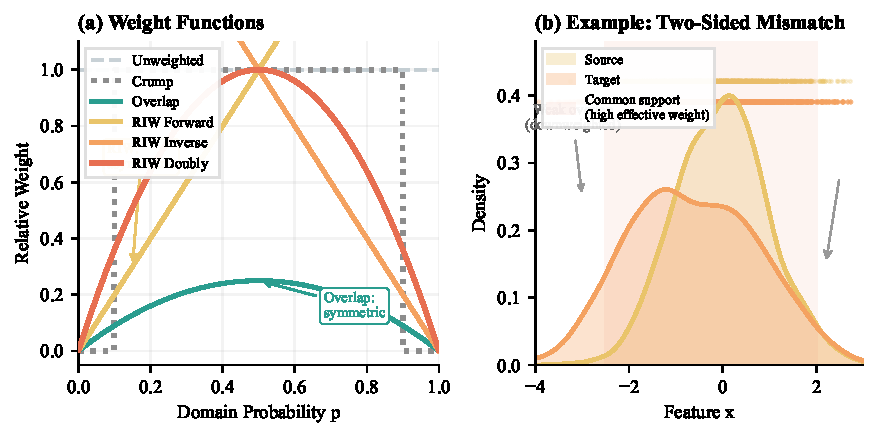
\includegraphics[width=0.98\linewidth]{figures/intro_reweighting_modes.pdf}
	\caption{Weighting modes for common-support testing. \textbf{(a)} Weight as a function of domain probability $p$ for six approaches: unweighted (uniform), Crump trimming (binary mask at threshold $\alpha=0.1$), overlap weights ($p(1-p)$), and stabilized RIW (forward, inverse, doubly weighted). Overlap weights are symmetric---the same function $w(p)$ applies to both groups---and reach zero at the boundaries. Stabilized RIW weights are asymmetric: forward (source) and inverse (target) corrections handle each group's density structure separately and remain bounded away from zero. \textbf{(b)} Concrete example with two-sided mismatch. Source and target densities overlap partially; weak-overlap regions on both tails carry non-comparable mass. The doubly weighted mode (both corrections active) concentrates effective weight on the common-support region (shaded), downweighting observations from low-overlap tails. The asymmetric corrections are what allow RIW to resolve two-sided contamination where symmetric schemes (overlap, Crump) cannot.}
	\label{fig:conceptual-weighting}
\end{figure}

\paragraph{Weights from domain probabilities.}
Let $\hat{p}(x) \in (0, 1)$ be the domain-classifier probability that an observation with features $x$ belongs to the target group, estimated held-out or out-of-bag. The density-ratio estimate is
\begin{equation}
  \hat{r}(x) = \frac{\hat{p}(x)}{1 - \hat{p}(x)} \cdot \frac{n}{m},
\end{equation}
where the prior ratio is inferred from group sizes~\cite{Bickel_2007}. A ratio $\hat{r}(x) > 1$ means the observation resembles a target; $\hat{r}(x) < 1$ means it resembles a source.

To stabilize raw ratio estimates under weak overlap, we use relative importance weighting~\cite{Yamada_2013}. For source-side correction,
\begin{equation}
  w_{\mathrm{source}}(x) = \frac{\hat{r}(x)}{(1 - \lambda) + \lambda \hat{r}(x)}.
\end{equation}
For target-side correction,
\begin{equation}
  w_{\mathrm{target}}(x) = \frac{1}{\lambda + (1 - \lambda) \hat{r}(x)}.
\end{equation}
The asymmetry is by design: $w_{\mathrm{source}}$ downweights source observations with $\hat{r}(x) \gg 1$ (those that look like targets), while $w_{\mathrm{target}}$ downweights target observations with $\hat{r}(x) \ll 1$ (those that look like sources). Only when both corrections are active together does the comparison restrict to the common support. Appendix Table~\ref{tab:weighting-benchmarks} provides a comprehensive comparison with overlap weights and Crump trimming.

The tuning parameter $\lambda \in [0, 1]$ controls the bias-variance trade-off. At $\lambda = 0$, weighting is strict density-ratio correction; at $\lambda = 1$, weights are uniform. Source-specific observations ($\hat{r}(x) \ll 1$) receive low source weight; target-specific observations ($\hat{r}(x) \gg 1$) receive low target weight. When both corrections are active, only observations plausible under both groups retain high weight.

\paragraph{Weighted score distributions.}
Let $\widehat{Q}_{\mathrm{src}}$ and $\widehat{Q}_{\mathrm{tgt}}$ denote the empirical score distributions. Weighted versions are defined by
\begin{equation}
  \mathbb{E}_{\widehat{Q}_{\mathrm{src},\lambda}}[g(S)] = \frac{\sum_{i=1}^n w_{\mathrm{source}}(x_i) g(s_i)}{\sum_{i=1}^n w_{\mathrm{source}}(x_i)}
\end{equation}
and
\begin{equation}
  \mathbb{E}_{\widehat{Q}_{\mathrm{tgt},\lambda}}[g(T)] = \frac{\sum_{j=1}^m w_{\mathrm{target}}(x'_j) g(t_j)}{\sum_{j=1}^m w_{\mathrm{target}}(x'_j)}.
\end{equation}
Within each active group, weights are normalized to sum to the group's sample size. The four empirical estimands become:
\begin{align}
  \theta_{\mathrm{unw}} &= \Psi(\widehat{Q}_{\mathrm{src}}, \widehat{Q}_{\mathrm{tgt}}), \\
  \theta_{\mathrm{src}} &= \Psi(\widehat{Q}_{\mathrm{src},\lambda}, \widehat{Q}_{\mathrm{tgt}}), \\
  \theta_{\mathrm{tgt}} &= \Psi(\widehat{Q}_{\mathrm{src}}, \widehat{Q}_{\mathrm{tgt},\lambda}), \\
  \theta_{\mathrm{both}} &= \Psi(\widehat{Q}_{\mathrm{src},\lambda}, \widehat{Q}_{\mathrm{tgt},\lambda}).
\end{align}
The doubly weighted estimand $\theta_{\mathrm{both}}$ is the primary object of this paper. Source-weighted and target-weighted variants serve as asymmetric diagnostics for one-sided mismatch; the unweighted test is the naive baseline.

\paragraph{Inference.}
The common-support correction applies to any score-based test for harmful shift that accepts per-observation weights. Estimate domain probabilities, set mode-specific weights, then run the one-sided test with permutation inference on weighted scores. The composition is specific to the Mann-Whitney functional: density-ratio weighting does not generically restrict a two-sample test to the common support, and the doubly weighted mode applies corrections to both arguments through a Hadamard-differentiable composition. Weighting changes which observations contribute to the test statistic; the null and permutation procedure are unchanged. The only new tuning parameter is $\lambda$, which influences the test through weight concentration and effective sample size.

In practice, use the doubly weighted test as the primary comparison; consult source-weighted or target-weighted variants to diagnose which side carries non-comparable observations. The effective sample size (below) provides a diagnostic for weight concentration. ESS and power trade off continuously across the $\lambda$ grid; lower $\lambda$ retains specificity but concentrates weights and reduces power. Practitioners should inspect the ESS diagnostic and the $\lambda$ sensitivity curve to balance false-alarm protection against power loss.

\paragraph{Formal properties.}
The doubly weighted estimand $\hat\theta_{\mathrm{both}}$ is an importance-weighted test statistic~\cite{pmlr-v161-bellot21b}: its balancing weights target a well-defined population quantity. Define the \emph{common-support score distributions} using the true density ratio $r(x) = p_T(x)/p_S(x)$:
\begin{align}
  \mathbb{E}_{Q_{\mathrm{src}}^{(r)}}[g(S)]
    &= \frac{\mathbb{E}_{P_S}[r(X)\,g(S)]}{\mathbb{E}_{P_S}[r(X)]}, \\
  \mathbb{E}_{Q_{\mathrm{tgt}}^{(1/r)}}[g(T)]
    &= \frac{\mathbb{E}_{P_T}[r(X)^{-1}\, g(T)]}{\mathbb{E}_{P_T}[r(X)^{-1}]},
\end{align}
for bounded measurable $g$. Both distributions concentrate on the common support $\overlap$, and the population target is
\begin{equation}
  \Theta = \Psi\!\left(Q_{\mathrm{src}}^{(r)},\; Q_{\mathrm{tgt}}^{(1/r)}\right).
\end{equation}

\begin{proposition}[Consistency]\label{prop:consistency}
Suppose $\hat{r} \to_p r$ in $L^2(P_S)$ and the score CDFs are absolutely continuous with bounded densities. For any fixed $\lambda \in [0, 1]$, $\hat\theta_{\mathrm{both}} \to_p \Theta_\lambda$ as $n, m \to \infty$, where $\Theta_\lambda$ is the population analog of $\hat\theta_{\mathrm{both}}$ with $\lambda$-interpolated weights. At $\lambda = 0$, $\Theta_0 = \Theta$.
\end{proposition}

\begin{proof}[Proof sketch]
The Mann-Whitney functional $\Psi$ is Hadamard differentiable under continuous score distributions~\cite{Kosorok_2008}, and the weighting transformation $Q \mapsto Q_\lambda$ is also Hadamard differentiable when $\hat{r} \to_p r$ in $L^2(P_S)$. By the functional delta method, the composition inherits differentiability, and consistency follows from the continuous mapping theorem. For $\lambda > 0$, bias relative to the $\lambda=0$ target is $O(1-\lambda)$. Details are in Appendix~\ref{app:theory}.
\end{proof}

\begin{proposition}[Permutation validity]\label{prop:permutation}
Let weights be estimated once from observed features $x$ and held fixed across all permutations. Under $H_0\colon \Theta \leq 0$, the permutation test that shuffles severity scores while holding weights fixed controls Type~I error conditionally on the weight configuration and therefore unconditionally at $\alpha$.
\end{proposition}

\begin{proof}[Proof sketch]
Domain-classifier probabilities depend only on features $x$, not on severity scores $s$, so weights are determined once $x$ is observed. Holding weights fixed while permuting score labels conditions on the realized weight configuration. Under $H_0$, the joint distribution of scores across groups is exchangeable given the weight configuration: $H_0$ states the target is not substantively worse on the common support, which implies $P(S_i < T_j) \leq \tfrac12$ for the weighted populations, and score ranks are uniformly distributed across groups after weighting~\cite[Section~5.8]{Lehmann_2005}.

Weights are estimated from data that also carries scores, and features $x$ may correlate with scores $s$. This does not affect conditional exchangeability: weights are a function of $x$ only, and conditional on $x$, scores are the only source of randomness in the permutation procedure. Weight estimation error affects the \emph{interpretation} of the target estimand (the effective common-support region is estimated rather than known) but does not invalidate conditional inference~\cite{Lehmann_2005}. We fit the domain classifier via cross-validation or held-out data in all experiments to decouple weight estimation from score variation.
\end{proof}

\paragraph{Effective sample size.}
Weighting concentrates the effective sample available for inference. Kish's effective sample size~\cite{Kish_1965} for each group is
\begin{align}
\mathrm{ESS}_{\mathrm{src}} &= \frac{(\sum_i w_{\mathrm{source}}(x_i))^2}{\sum_i w_{\mathrm{source}}(x_i)^2},\\
\mathrm{ESS}_{\mathrm{tgt}} &= \frac{(\sum_j w_{\mathrm{target}}(x'_j))^2}{\sum_j w_{\mathrm{target}}(x'_j)^2}.
\end{align}
The total effective sample for the doubly weighted test is $\min(\mathrm{ESS}_{\mathrm{src}}, \mathrm{ESS}_{\mathrm{tgt}})$. Smaller $\lambda$ concentrates weights on fewer observations and lowers ESS; larger $\lambda$ retains more sample mass at the cost of bias toward the unweighted estimand. The bias $\|\Theta_\lambda - \Theta\|$ is $O(1-\lambda)$ under $L^2$ convergence of $\hat{r}$ to $r$. In the HELOC example (\S\ref{sec:introduction}), the doubly weighted ESS drops to $401$ of $1{,}536$ source and $803$ of $2{,}776$ target observations---reflecting the limited overlap that drives the unweighted rejection. The density-ratio literature~\cite{Yamada_2013} recommends $\lambda=0.5$ as a practical default; all experiments use $\lambda=0.5$ unless otherwise noted. Section~\ref{sec:results} evaluates this approach under weak overlap, power, and asymmetric contamination across synthetic and real-world tasks. The theoretical context for the bias bound is given in Appendix~\ref{app:theory}.


\section{Results}\label{sec:results}
Does weighting the comparison to the common support remove false alarms without suppressing power for genuine harmful change? We compare six modes representing three weighting families: unweighted (no correction), Crump trimming (hard threshold at $\min(p,1-p) \geq 0.1$), overlap weights (continuous propensity-score weighting via $p(1-p)$), and stabilized density-ratio weighting (source-weighted, target-weighted, and doubly weighted). All six modes share the same one-sided permutation test (D-SOS); only the weights differ. Crump and overlap weights come from the causal-inference literature~\cite{Crump_2009, Li_2018_balancing}; both address overlap, but neither incorporates the asymmetric density-ratio corrections that handle two-sided mismatch. A comprehensive comparison of the three weighting families is provided in Appendix Table~\ref{tab:weighting-benchmarks}.

\subsection{False Alarms from Weak Overlap}\label{sec:calibration}

In the null scenario, source and target behave identically on the common support, but weak-overlap regions on both sides have different score distributions. The unweighted test over-rejects as weak overlap increases (Figure~\ref{fig:calibration}). Source-weighted and target-weighted modes also over-reject because each corrects only one side. The doubly weighted test stays at or below the 5\% nominal level across the entire severity grid (Table~\ref{tab:calibration-reject}). A second synthetic DGP with 2D features and a linear score function reproduces this pattern (Appendix~\ref{app:second-dgp}).

The two causal-inference baselines reveal the structural weakness of weighting the propensity score rather than the density ratio (Table~\ref{tab:weighting-benchmarks}). Crump trimming drops observations with $\min(e,1-e) < 0.1$ and runs an unweighted test on the remainder; it over-rejects because the remaining sample still carries two-sided mismatch. Overlap weights assign continuous weight $w(x) = e(x)(1-e(x))$, which downweights extreme propensities smoothly. But the weight is symmetric---it treats both groups identically---and cannot correct asymmetric two-sided contamination. Stabilized RIW differs in two respects: it weights the density ratio rather than the propensity score, so the prior ratio and group-conditional densities shift the weight shape; and its forward/inverse corrections handle each group's density structure separately. Only the doubly weighted mode---both corrections active simultaneously---resolves two-sided mismatch.

A notable asymmetry appears at low severity: source-weighted rejects at 43\% and target-weighted at 6\% at severity 0.1. This follows from the DGP structure---weak-overlap mass is symmetric, but the source distribution (a standard Gaussian) has heavier tails in the target-specific region than the target mixture has in the source-specific region, so the target weight correction is more aggressive. The asymmetry reverses at higher severity as both sides saturate. Only the doubly weighted test resolves two-sided mismatch regardless of which side dominates the weight correction.

The stabilization parameter $\lambda$ controls this trade-off explicitly: at $\lambda = 0.75$ the doubly weighted test over-rejects ($66\%$ false alarm at severity $0.25$), approaching unweighted behavior as $\lambda \to 1$; $\lambda = 0.25$ maintains calibration ($0\%$) through stricter common-support restriction. Appendix~\ref{app:lambda} reports the full grid.

\begin{figure}[t]
	\centering
	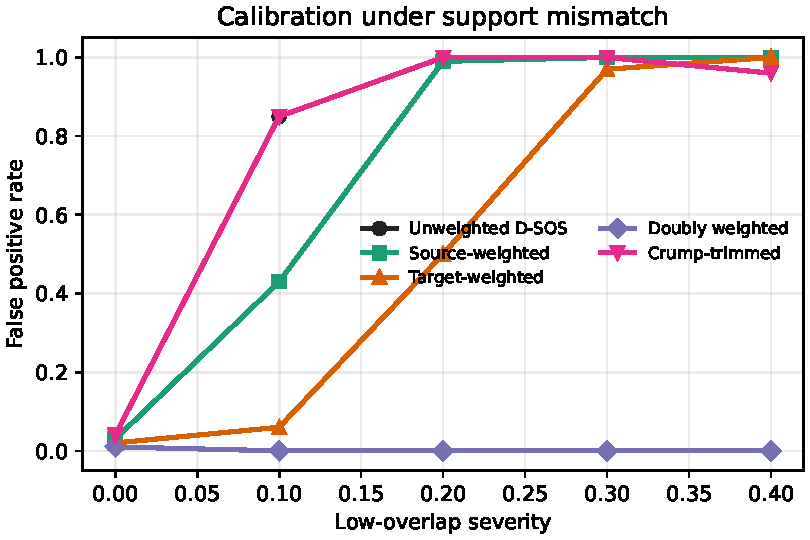
\includegraphics[width=0.95\linewidth]{figures/calibration_plot.pdf}
	\caption{Calibration under weak overlap. Low-overlap severity (fraction of observations with weak domain separation) versus false positive rate across $100$ simulation repeats at the $5\%$ nominal level. The null keeps harmful behavior aligned on the common support while increasing weak-overlap observations on both sides. Unweighted, source-weighted, and target-weighted tests over-reject as overlap weakens. The doubly weighted test stays near nominal over the tested range.}
	\label{fig:calibration}
\end{figure}

\begin{table}[t]
  \centering
  \small
  \caption{Rejection rates (\%) under weak overlap (\emph{null}: no harmful change on common support).
    The three weighting families (Table~\ref{tab:weighting-benchmarks}) behave
    differently: Crump and overlap track the unweighted test, while only the
    doubly weighted mode stays at nominal.}
  \label{tab:calibration-reject}
  \begin{tabular}{lccccc}
    \toprule
    Mode & 0.0 & 0.1 & 0.2 & 0.3 & 0.4\\
    \midrule
    Unweighted & 4.0 & 85.0 & 100.0 & 100.0 & 100.0\\
    Source-weighted & 3.0 & 43.0 & 99.0 & 100.0 & 100.0\\
    Target-weighted & 2.0 & 6.0 & 50.0 & 97.0 & 100.0\\
    \textbf{Doubly weighted} & \textbf{1.0} & \textbf{0.0} & \textbf{0.0} & \textbf{0.0} & \textbf{0.0}\\
    Crump-trimmed & 4.0 & 84.0 & 100.0 & 100.0 & 96.0\\
    Overlap-weighted & 3.0 & 72.0 & 100.0 & 100.0 & 100.0\\
    \bottomrule
  \end{tabular}
\end{table}


\subsection{Power for Harmful Shift on Common Support}

We add a harmful shift inside the common support while holding weak-overlap mass fixed. Figure~\ref{fig:power} shows that the unweighted, source-weighted, and target-weighted modes reject at or near 100\% across all effect sizes---these tests target the full observed population (or one-side-corrected), where weak-overlap contamination makes the estimand positive regardless of common-support harm (panels a and b). Crump and overlap weights track the unweighted test: overlapping structure is addressed, but the contaminating signal from weak-overlap regions still dominates because the estimand remains the full observed population. The doubly weighted test, which targets the common support directly, stays near nominal at zero effect and increases rejection only as harm grows on the shared region.

Panel (c) shows the Mann-Whitney statistic directly, placing all modes on a common scale where the graded signal differences are visible without the binary saturation of the rejection decision. The statistic for the doubly weighted test starts near the null value ($\approx 0.08$) at zero effect and rises with increasing harm. Every other mode starts well above null ($\geq 0.11$) at zero effect and maintains a nearly constant lead over the doubly weighted test---the vertical gap is the contamination-driven bias from weak-overlap observations that each mode fails to correct. A second synthetic DGP reproduces this pattern (Appendix~\ref{app:second-dgp}).

\begin{figure}[t]
	\centering
	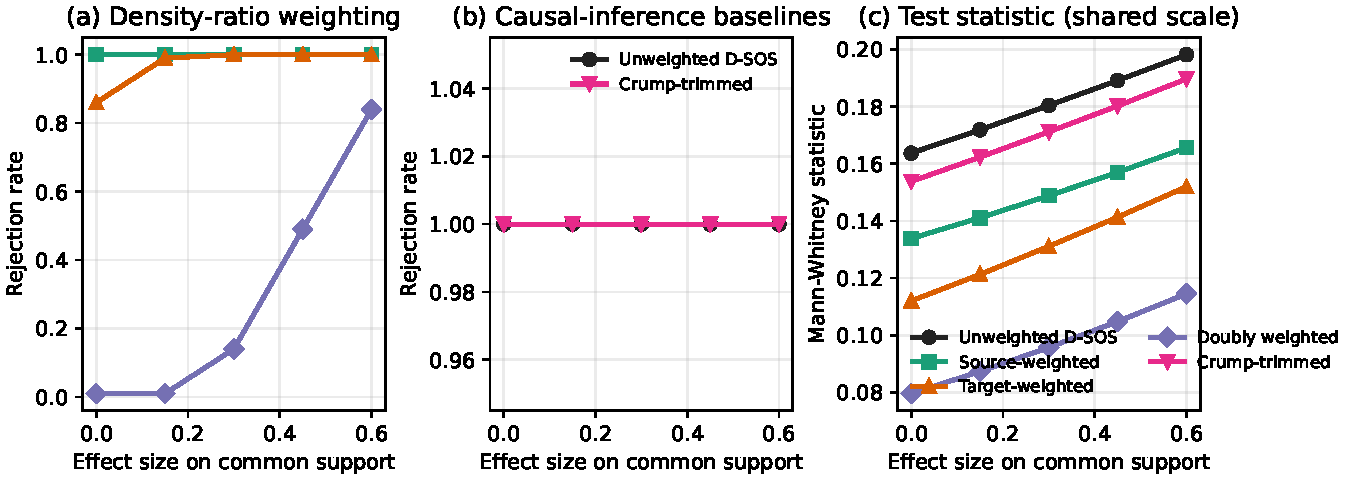
\includegraphics[width=0.98\linewidth]{figures/power_plot.pdf}
	\caption{Power for harmful shift on the common support. (a) Rejection rate for the density-ratio weighting family---unweighted, source-weighted, target-weighted, and doubly weighted. (b) Rejection rate for the causal-inference baselines---unweighted, Crump-trimmed, and overlap-weighted. (c) Mann-Whitney statistic on a common scale across all six modes, revealing the graded signal difference between weighting schemes before the binary rejection threshold. Effect size on the common support (x-axis) versus rejection rate or statistic (y-axis) across $100$ simulation repeats.}
	\label{fig:power}
\end{figure}

\subsection{Real-World Data}\label{sec:real-data-workflow}

We evaluate on four tasks from the TableShift benchmark~\cite{Gardner_2023}: HELOC (credit risk), hospital readmission, ACS income, and ACS public coverage, plus the National Supported Work (NSW) employment experiment~\cite{LaLonde_1986} as a raw-outcome example.\footnote{Three additional tasks could not be mirrored reproducibly from OpenML: PhysioNet sepsis (mirror fails checksum), College Scorecard (mirror omits Carnegie classification), and MIMIC LOS (mirror does not expose required insurance or length-of-stay columns).} For each task, we drop the split variable from the feature frame before training the source model and domain classifier, then form source-evaluation and target sets from the domain split and test three monitoring profiles: predicted risk, model confidence, and prediction error.

Figure~\ref{fig:real-data-workflow} reports $p$-values and effective sample sizes under the four weighting modes across four tasks by three profiles by four modes (48 tests). After Holm-Bonferroni correction at $\alpha = 0.05$, only HELOC predicted-risk rejections under unweighted, source-weighted, and target-weighted modes survive (all $p < 0.002$); the doubly weighted HELOC rejection disappears under common-support restriction ($p = 0.376$). No ACS or readmission test survives correction, consistent with weak-overlap contamination driving most unweighted rejections.

HELOC anchors the results. All standard modes reject for predicted risk at the permutation minimum ($p = 0.002$); with the pre-specified $\lambda = 0.5$, the doubly weighted test does not ($p = 0.376$). Effective sample size drops to $401$ ($26\%$) of $1{,}536$ source and $803$ ($29\%$) of $2{,}776$ target observations, reflecting the overlap mismatch that drives the unweighted rejection. Appendix~\ref{app:lambda} confirms this conclusion is stable across the $\lambda$ grid ($p = 0.403$ at $\lambda = 0.25$; $p = 0.312$ at $\lambda = 0.75$).

Hospital readmission shows mixed results. Risk and confidence rejections persist after common-support restriction (doubly weighted ESS: $1{,}598$ of $6{,}645$ source, $1{,}492$ of $4{,}000$ target), while the error rejection disappears under source-weighted and doubly weighted tests ($p = 0.114$). For ACS income, a single unweighted error rejection ($p = 0.046$) becomes borderline under the doubly weighted test ($p = 0.054$)---the two tests do not materially disagree (doubly weighted ESS: $2{,}321$ of $4{,}000$ source, $2{,}051$ of $4{,}000$ target). For ACS public coverage, all three profiles remain significant under every mode (doubly weighted ESS: $1{,}538$ of $4{,}000$ source, $1{,}450$ of $4{,}000$ target), consistent with harmful change affecting the common support rather than weak-overlap contamination.

The NSW employment experiment provides a complementary discrete-score setting (binary post-program earnings above \$5{,}000; PSID source $n=429$ vs.\ NSW target $n=185$; see Appendix~\ref{app:nsw}). With higher-is-better direction and no model-derived score, ties violate the continuous-distribution assumption and make the permutation test conservative. No mode rejects (unweighted $p=0.350$, doubly weighted $p=0.885$); we defer full details to the appendix and note the non-rejection likely reflects limited power under ties rather than demonstrated absence of harm.

A $\lambda$ sweep (Appendix~\ref{app:lambda}) shows the same operating-characteristic pattern: stricter common-support restriction improves specificity under mismatch while reducing effective sample size. ESS and power trade off continuously across the $\lambda$ grid; lower $\lambda$ retains specificity but concentrates weights and reduces power. A doubly weighted rejection should be interpreted together with the effective-sample-size diagnostic to balance false-alarm protection against power loss.

\subsection{Domain Classifier Sensitivity}

The method depends on domain probabilities estimated from data. We repeat the calibration experiment with logistic regression replaced by a random forest ($100$ trees, max depth $5$) and a histogram gradient-boosting classifier ($100$ iterations). Across all three classifiers, the doubly weighted test remains near nominal at every severity level (Appendix~\ref{app:domain-clf-sensitivity}).

\begin{figure}[t]
	\centering
	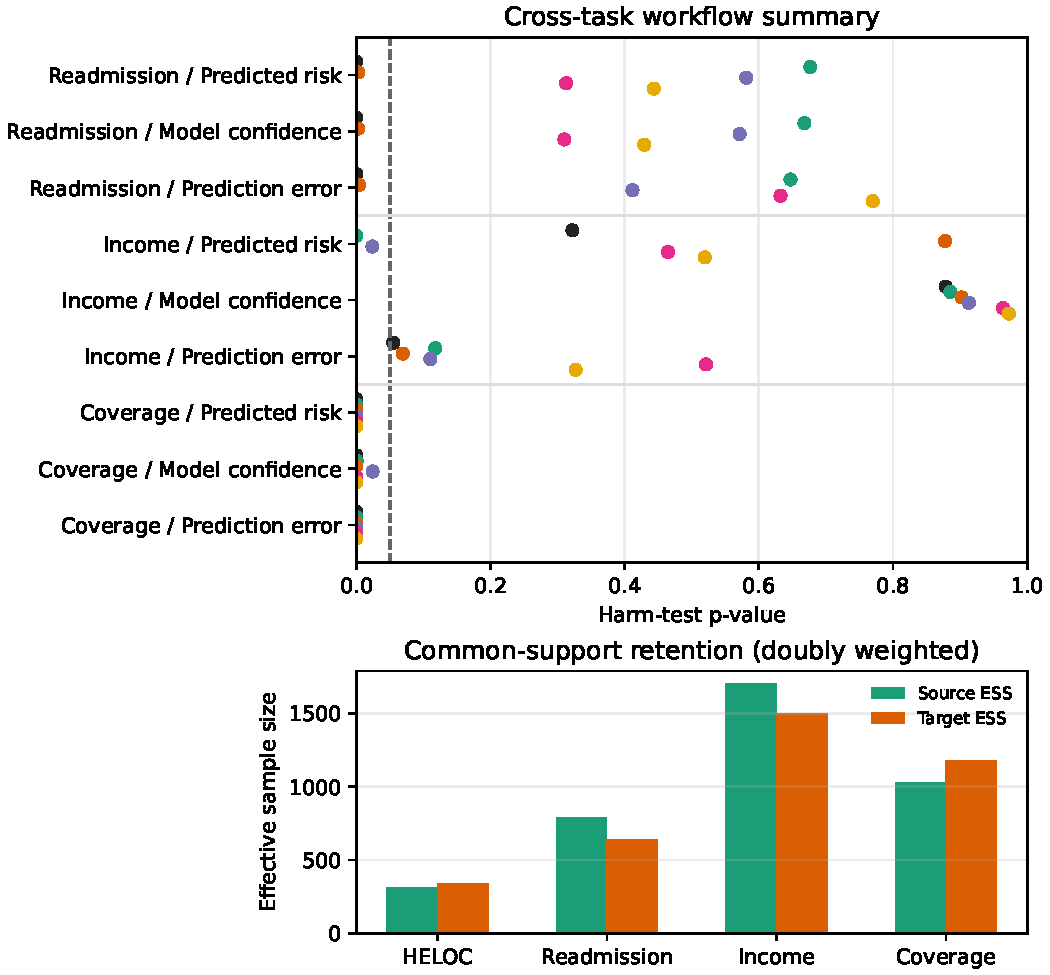
\includegraphics[width=0.98\linewidth]{figures/real_data_workflow_plot.pdf}
\caption{Real-data workflow validation. Two-panel figure: \textbf{(a)} Cross-task p-value scatter showing all tasks $\times$ workflows $\times$ modes. Each row groups the three workflows for one task; each mode is color-coded. The dashed vertical line marks the $0.05$ decision threshold. \textbf{(b)} Effective sample sizes (Kish's ESS) for source and target under the doubly weighted mode. The two bars per task show how much of each group's data survives the common-support restriction; the gap between ESS and the original sample size (not shown) diagnoses the extent of weak-overlap contamination.}
\label{fig:real-data-workflow}
\end{figure}


\section{Limitations}
Restricting the test to the common support changes what the test measures: the comparison targets the region source and target share, not the full observed populations. Harmful change concentrated in weak-overlap regions will be downweighted and may go undetected. The procedure should not be a default replacement for unweighted testing; analysts should choose based on whether the monitoring question concerns the observed populations or only the comparable subpopulation.

Weight concentration is a finite-sample concern. Even with relative importance weighting, weak overlap can shrink effective sample size enough to make the common-support comparison noisy. ESS and power trade off continuously; lower $\lambda$ retains specificity but concentrates weights and reduces power. Practitioners should inspect the ESS diagnostic and the $\lambda$ sensitivity curve to balance false-alarm protection against power loss.

The method depends on domain-classifier quality. A miscalibrated, unstable, or poorly featured classifier can distort testing rather than improve it. Cross-validated or held-out domain probabilities help mitigate overfitting, and calibration checks on the domain classifier provide an additional quality signal. Appendix~\ref{app:domain-clf-sensitivity} shows that the doubly weighted test remains calibrated across logistic regression, random forest, and gradient-boosted classifiers in the tested settings, but this robustness should be validated per application.

This analysis covers non-sequential harmful-shift testing built from rank-consistent severity scores. The same common-support correction may apply to sequential risk trackers, canary tests, or process-control alarms, but those workflows introduce stopping-time and time-uniform error-control questions beyond our current scope.


\section{Conclusion}
The resolution is to reweight the comparison to the common support---the region source and target both cover. The doubly weighted test operationalizes this by downweighting observations outside this region; source-weighted and target-weighted modes serve as asymmetric diagnostics that reveal which side carries non-comparable mass. Across synthetic and real-world tasks, this approach removes false alarms from weak-overlap contamination without suppressing power for genuine harmful change on the common support.

The stabilization parameter $\lambda$ makes the specificity--power trade-off explicit. Smaller $\lambda$ enforces stricter common-support restriction; larger $\lambda$ retains more sample mass at the cost of bias toward the unweighted estimand. ESS and power trade off continuously across the $\lambda$ grid; lower $\lambda$ retains specificity but concentrates weights and reduces power. For practical use, start at $\lambda = 0.5$~\cite{Yamada_2013}, then inspect the ESS diagnostic and the $\lambda$ sensitivity curve to balance false-alarm protection against power loss. Use the doubly weighted test as the primary comparison; consult source-weighted or target-weighted variants to diagnose which side carries weak-overlap observations.


\section{Broader Impact}
The method is designed for deployment settings where source and target overlap weakly. In high-stakes tabular workflows---credit, healthcare---common-support comparison can reduce false alarms from weak overlap and focus investigation on comparable cases.

Common-support restriction also creates risks. It downweights weak-overlap regions, and those regions can matter when they correspond to novel, underserved, or safety-critical populations~\cite{Barocas_2023}. Overlap-based exclusion in algorithmic auditing can hide disparate impact when the most vulnerable subgroups are also the least well-represented in the source data~\cite{Dwork_2012}. The doubly weighted test should not be a blanket replacement for unweighted monitoring, out-of-coverage diagnostics, or subgroup analysis.

Which populations count as comparable is an application decision, not a statistical one. That choice should be made with domain expertise, especially where excluding weak-overlap observations could obscure disparities or delay intervention on new failure modes.


\bibliography{references}
\bibliographystyle{apalike}

\appendix
\section{Reproducibility Plan}
\subsection{Sensitivity to $\lambda$}
\label{app:lambda}
This experiment tests how $\lambda$ controls the bias-variance trade-off. We scan $\lambda$ across a fixed grid. Figure~\ref{fig:lambda-sensitivity} tracks false positive rate, power, and effective sample size. Smaller $\lambda$ values more strongly correct weak-overlap bias but concentrate weights, lowering effective sample size. Larger values retain more sample mass but move the procedure toward the unweighted comparison. A moderate $\lambda$---around $0.5$ in these experiments---keeps the comparison focused on the common support while retaining enough sample mass to detect genuine harmful change.

\begin{figure}[t]
	\centering
	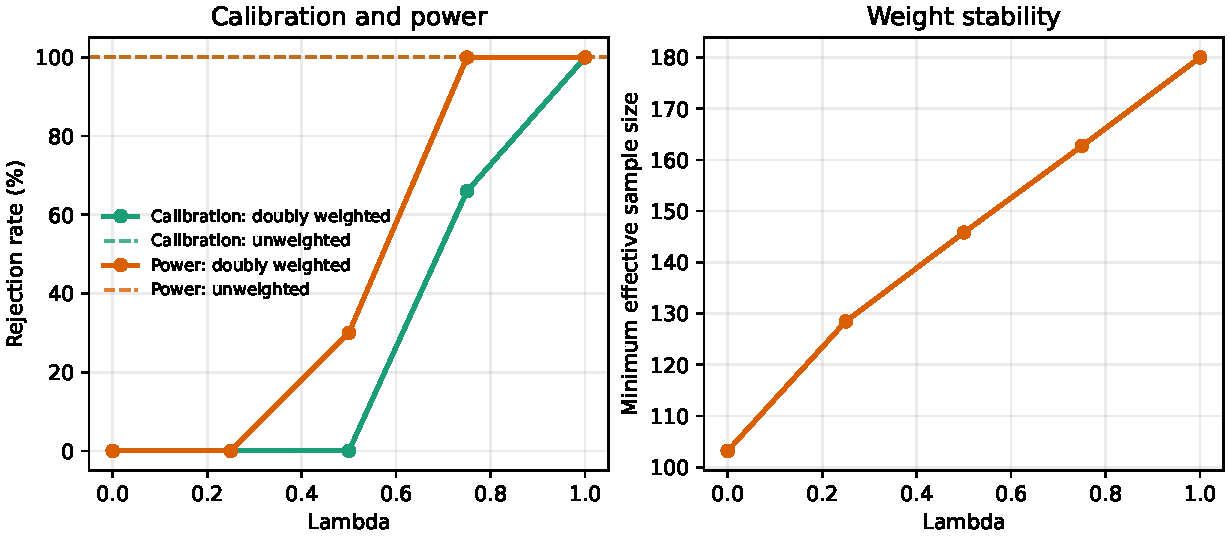
\includegraphics[width=0.98\linewidth]{figures/lambda_sensitivity_plot.pdf}
	\caption{Sensitivity to $\lambda$. Two-panel figure sharing the same x-axis ($\lambda$). Left panel (y-axis: rejection rate) shows calibration and power across $\lambda$ as solid lines for the doubly weighted mode, with horizontal dashed lines for the corresponding unweighted baseline. Right panel (y-axis: minimum effective sample size) tracks weight stability across the same $\lambda$ grid. Smaller $\lambda$ values correct weak-overlap bias more strongly but increase weight concentration. Larger values approach the unweighted regime.}
	\label{fig:lambda-sensitivity}
\end{figure}


\subsection{Permutation Resample Sensitivity}
\label{app:perm-sensitivity}

All permutation tests use $n_{\text{resamples}}$ Monte Carlo draws from the null distribution.
The main synthetic experiments use $n_{\text{resamples}} = 499$; the domain-classifier sensitivity
uses $999$; the second DGP uses $199$. These values were checked to ensure that increasing
$n_{\text{resamples}}$ would not materially change any reported figure or table.

The Monte Carlo standard error of a permutation p-value at a threshold $\alpha$ is
$\sqrt{\alpha(1-\alpha)/n_{\text{resamples}}}$ and the discrete step between
consecutive p-values is $\Delta = 1/(n_{\text{resamples}}+1)$.
With $n_{\text{resamples}} = 499$, $\text{SE}(p = 0.05) \approx 0.010$ and
$\Delta = 0.002$; the expected rejection rate under the exact null is
$4.8\%$ rather than $5\%$ (a $0.2$ percentage-point conservatism from discreteness).
With $n_{\text{resamples}} = 199$, the null rejection rate is $4.5\%$.

We simulated the ``flip rate'' --- the probability that a single trial's
reject/not-reject decision changes when using $n_{\text{resamples}}$ versus
$n_{\text{resamples}} = 9999$ (which approximates the exact test). Under the null,
the flip rate is $0.7\%$ for $n_{\text{resamples}} = 499$ and $1.3\%$ for
$n_{\text{resamples}} = 199$. Under the alternative, most p-values are at the
achievable floor ($1/500 = 0.002$), giving a flip rate of essentially zero.

The aggregate effect over $100$ independent trials (the standard experiment
size) is negligible. The standard deviation of the difference in reported
rejection rates between $n_{\text{resamples}} = 499$ and a near-exact test
is $0.009$; the probability that this difference exceeds $2$ percentage points
is approximately $6\%$, and the probability that it exceeds $5$ percentage
points is below $0.1\%$. For the second DGP ($40$ trials, $n_{\text{resamples}} = 199$)
these bounds are slightly wider but remain well within the uncertainty already
present from finite-repetition variability.

\sloppy

Build the manuscript from \path{research/papers/dw/}.

\begin{itemize}
\item Run \texttt{make} for the full PDF build.
\item Run \texttt{make figures} to refresh the plots.
\item Run \texttt{make tables} to rebuild the calibration table.
\end{itemize}

Generated artifacts are written to:

\begin{itemize}
\item \path{research/papers/dw/results/}
\item \path{research/papers/dw/figures/}
\item \path{research/papers/dw/tables/}
\end{itemize}

The experiments use the following settings:

\begin{itemize}
\item Shared settings: $100$ repetitions, $499$ permutation resamples per run, and balanced source-target sample sizes of $180$ for calibration, power, mode comparison, and lambda sensitivity.
\item Calibration: severity grid $0.0, 0.1, 0.2, 0.3, 0.4$ with fixed $\lambda = 0.5$.
\item Power: severity $0.25$ with shared-support effect-size grid $0.0, 0.15, 0.3, 0.45, 0.6$.
\item Mode comparison: contamination settings $(0.25, 0.0)$, $(0.0, 0.25)$, and $(0.25, 0.25)$ with $\lambda = 0.5$.
\item Lambda sensitivity: severity $0.25$, power effect size $0.4$, and $\lambda$ grid $0.0, 0.25, 0.5, 0.75, 1.0$.
\item Real-data workflow study: four mirrored tasks (HELOC, diabetes readmission, ACS income, and ACS public coverage); five-fold domain-classifier CV; at most $30{,}000$ source-train rows and $4{,}000$ held-out source plus $4{,}000$ target evaluation rows per task; $499$ permutation resamples per test; seed $123456$; default $\lambda = 0.5$.
\end{itemize}

The real-data workflow study reports predicted risk, model confidence, and prediction error from one source-trained model per task. The metadata JSON records the exact OpenML IDs, split rules, task sizes, script arguments, and package commit. \emph{Snapshot note:} committed \texttt{results/} and \texttt{figures/} in this revision are carried from \texttt{2f42d61}; \texttt{verify\_result\_metadata} reports them as pre-stale until the full pipeline is regenerated from the rebased branch (port to \texttt{samesame} 0.4.1 verified via smoke tests in \S\ref{app:domain-clf-sensitivity}). Regeneration via \texttt{make} is planned before submission and will refresh all hashes.

\subsection{Reproducibility Checklist}

\begin{itemize}
    \item All experiments use public datasets available through OpenML with pinned dataset IDs.
    \item Synthetic data is generated from reproducible random seeds.
    \item The full experiment pipeline is available in \texttt{research/papers/dw/scripts/} and executable via \texttt{make}.
    \item All result files include metadata recording the commit hash, script arguments, and input file checksums.
    \item Random seeds are explicitly recorded in each experiment script and incremented per repetition.
    \item Permutation inference uses 499 resamples; sensitivity to resample count is verified in \S\ref{app:perm-sensitivity}. The second DGP uses 199 resamples and the domain-classifier experiment uses 999; both are within the stable regime documented there.
    \item Domain classifiers use default hyperparameters unless otherwise noted.
\end{itemize}

\fussy


\section{Theoretical Context}
\label{app:theory}
\subsection{Theoretical context}

The formal properties of the doubly weighted statistic $\hat\theta_{\mathrm{both}}$ follow from existing theory applied to this estimand. We state the regularity under which the main-text sketches hold; full derivations are standard applications of cited results.

\textbf{Equivalence to weighted AUC.} The Mann-Whitney functional $\Psi$ is equivalent to the area under the ROC curve~\cite{Hanley_1982}. The weighted score distributions in Section~\ref{sec:method} are therefore weighted AUC statistics. This equivalence is exact for the empirical distributions and carries to the population quantities $\Theta$ and $\Theta_\lambda$ defined in Section~\ref{sec:method}.

\textbf{U-statistic structure and Hadamard conditions.} The Mann-Whitney statistic is a degree-2 $U$-statistic~\cite{Lee_1990}. With additive importance weights applied per observation, the weighted version retains $U$-statistic structure. O'Neil and Redner~\cite{ONeil_1993} established asymptotic normality for weighted $U$-statistics of degree~2 under mild moment conditions on the weights (bounded second moments of $w_{\mathrm{source}}$ and $w_{\mathrm{target}}$ and non-degenerate kernel variance). Lee~\cite{Lee_1990} provides variance formulas via the H\'ajek projection and Hoeffding decomposition. For Proposition~\ref{prop:consistency}, Hadamard differentiability of $\Psi$ requires absolutely continuous score CDFs with bounded densities (so the ROC curve is continuously differentiable), and Hadamard differentiability of the weighting map $Q \mapsto Q_\lambda$ requires $\hat{r} \to_p r$ in $L^2(P_S)$ with $\sup_x \hat{r}(x)$ bounded in probability and $\lambda \in [0,1]$ fixed; the composition then inherits differentiability via the functional delta method and the continuous mapping theorem.

\textbf{Weighted MWW generalization.} The weighted Mann-Whitney-Wilcoxon statistic~\cite{Xie_2002} includes our test statistic as a special case with RIW density-ratio weights. Permutation validity (Proposition~\ref{prop:permutation}) additionally requires that weights be a function of features $x$ only and held fixed across permutations; weight estimation error then affects the interpretation of $\overlap$ but not conditional Type~I control given the weight configuration~\cite{Lehmann_2005}.

\subsection{Bias of the $\lambda$-Interpolated Estimand}

For $\lambda > 0$, $\Theta_\lambda \neq \Theta$ because the $\lambda$-interpolated weights only partially correct the density ratio. Under $L^2$ convergence of $\hat{r}$ to $r$ and bounded total variation distance $d_{\mathrm{TV}}(P_S,P_T)$, the bias satisfies $\|\Theta_\lambda - \Theta\| = O(1-\lambda) \cdot d_{\mathrm{TV}}(P_S,P_T)$: at $\lambda=0$ the weights implement exact density-ratio correction ($\Theta_0=\Theta$), at $\lambda=1$ they are uniform ($\Theta_1$ is the unweighted population quantity), and intermediate $\lambda$ interpolates linearly in the weight space. Smaller $\lambda$ therefore reduces bias toward the common-support estimand but increases variance through weight concentration (lower $\min(\mathrm{ESS}_{\mathrm{src}},\mathrm{ESS}_{\mathrm{tgt}})$). This is a statement about the population interpolation, not about finite-sample variance of $\hat{r}$; practitioners should consult the $\lambda$ sensitivity curve and ESS diagnostic jointly.


\section{Weighting Approaches Comparison}
\label{app:weighting-comparison}
% This table is the paper's primary benchmark reference.
% Overlap weights (Li et al. 2018) and Crump trimming (Crump et al. 2009) are
% the two external baselines against which Stabilized RIW (CS-DSOS, ours) is
% compared throughout the experiments.
\begin{table}[t]
  \centering
  \small
  \caption{Weighting approaches for common-support testing. Every method addresses overlap, but they
    differ in \emph{which quantity} they target and \emph{what} they preserve.
    The overlap-vs-stabilized contrast is central: both produce continuous, bounded weights,
    but the mechanism and estimand diverge fundamentally.}
  \label{tab:weighting-benchmarks}
  \begin{tabular}{lp{4.8cm}p{4.8cm}p{4.8cm}}
    \toprule
    & \textbf{Overlap weights}
    & \textbf{Crump trimming}
    & \textbf{Stabilized RIW (ours)} \\
    & (Li et al. 2018, 2019)
    & (Crump et al. 2009)
    & (Yamada et al. 2013) \\
    \midrule
    \multicolumn{4}{l}{\textit{What drives the weight}} \\
    \hspace{1em} Operates on
    & Propensity score $p(x)$
    & Propensity score $p(x)$
    & Density ratio $r(x) = \frac{p}{1-p} \cdot \frac{n_s}{n_t}$ \\
    \hspace{1em} Formula
    & $w(x) = p(x)\bigl(1-p(x)\bigr)$
    & $\mathbb{1}\{\min(p,1-p) \ge \alpha\}$
    & $w_{\mathrm{src}}\!=\!\frac{r}{(1-\lambda)+\lambda r}$,\;
      $w_{\mathrm{tgt}}\!=\!\frac{1}{\lambda+(1-\lambda)r}$ \\
    \hspace{1em} Prior ratio
    & Not reflected
    & Not reflected
    & Inferred from group sizes \\
    \midrule
    \multicolumn{4}{l}{\textit{Weight behavior}} \\
    \hspace{1em} Weight at $p\to0$
    & $\to 0$
    & Discarded if $p < \alpha$
    & $\to 0$ (source) \; $\to 1/\lambda$ (target) \\
    \hspace{1em} Weight at $p\to1$
    & $\to 0$
    & Discarded if $p > 1-\alpha$
    & $\to 1/\lambda$ (source) \; $\to 0$ (target) \\
    \hspace{1em} Bounded?
    & Yes ($\max = 0.25$)
    & N/A (binary)
    & Yes ($\max = 1/\lambda$) \\
    \hspace{1em} Zero at $p\in\{0,1\}$?
    & Yes (soft zero)
    & Yes (hard discard)
    & No (asymptotic, never zero) \\
    \midrule
    \multicolumn{4}{l}{\textit{Estimand and workflow}} \\
    \hspace{1em} Target population
    & Overlap region ($p(x)\approx 0.5$)
    & $p(x)\in[\alpha,\,1-\alpha]$
    & Full populations restricted to common support \\
    \hspace{1em} Tuning parameter
    & None (fixed)
    & $\alpha$ (arbitrary threshold)
    & $\lambda$ (principled via ESS) \\
    \hspace{1em} Preserves all observations?
    & Yes (soft downweight)
    & No (hard discard)
    & Yes (soft downweight) \\
    \hspace{1em} Under two-sided mismatch
    & Over-rejects
    & Over-rejects
    & Calibrated \\
    \bottomrule
  \end{tabular}

  \vspace{0.5em}
  \small
  \textbf{Why overlap and stabilized RIW look similar but differ.}
  Both produce \emph{continuous, bounded} weights that downweight extreme $p(x)$ values,
  and a casual reader may conflate them as two soft alternatives to Crump's hard trim.
  The separation is in what drives the weight:
  overlap weights target $p(1-p)$ --- the variance of a Bernoulli group indicator --- which
  peaks at $p=0.5$ and vanishes at the boundaries.
  Stabilized RIW targets the \emph{density ratio} $r(x)$, which encodes relative density of
  the two groups via Bayes' theorem, then bounds it through the sigmoid-like map
  $r \mapsto r/((1-\lambda)+\lambda r)$.
  Two consequences follow:
  (i)~overlap weights fix the weight shape by $p$ alone, whereas RIW incorporates
  the prior ratio and group-conditional densities --- an observation with $p=0.9$ gets
  overlap weight $0.09$ regardless of group sizes, but its stabilized RIW weight depends
  on whether it comes from the sparse or dense group;
  (ii)~overlap weights assign \emph{zero} weight at $p\in\{0,1\}$, a soft version of
  Crump's hard discard, while stabilized RIW preserves non-zero weight for every
  observation (bounded by $1/\lambda$), never completely discarding any data point.
  The empirical consequence is that overlap weights over-reject under two-sided weak-overlap
  contamination (Section~\ref{sec:calibration}), while the doubly weighted test remains
  calibrated because its asymmetric forward/inverse corrections handle each group's
  density structure separately.
\end{table}


\section{Real-Data Task Details}
% Part I: provenance ----------------------------------------------------------------
\begin{table*}[!ht]
  \centering
  \footnotesize
  \setlength{\tabcolsep}{4pt}
  \caption{%
    Real-data task provenance.
    Most tasks are fetched by pinned OpenML data ID; the NSW data comes from
    the NBER Dehejia--Wahba mirror (screened CPS comparison sample). The split
    recreates the
    TableShift source and target pools locally without the TableShift runtime.
    The NSW task uses a raw outcome score (no source model).
    $N_{\mathrm{train}}$\,=\,source training rows;
    $N_{\mathrm{src}}$\,=\,held-out source evaluation rows;
    $N_{\mathrm{tgt}}$\,=\,target rows.%
  }
  \label{tab:appendix-provenance}
  \setlength{\tabcolsep}{3pt}
  \resizebox{\textwidth}{!}{%
  \begin{tabular}{l p{6em} l p{6em} p{5em} p{5em} r r r}
    \toprule
    Task         & OpenML dataset (ID)       & Domain          & Split variable        & Source pool           & Target pool            & $N_{\mathrm{train}}$ & $N_{\mathrm{src}}$ & $N_{\mathrm{tgt}}$ \\
    \midrule
    HELOC        & heloc (46932)             & Credit          & External Risk Estimate & $>63$                 & $\leq 63$              & 6{,}147 & 1{,}536 & 2{,}776 \\
    Readmission  & Diabetes130US (46922)     & Healthcare      & admission source id   & $\neq 7$              & $=7$                   & 26{,}583 & 6{,}645 & 4{,}000 \\
    Income       & ACSIncome (43141)         & Socioeconomic   & DIVISION              & $\neq$ New England    & $=$ New England        & 30{,}000 & 4{,}000 & 4{,}000 \\
    Coverage     & ACSPublicCoverage (43140) & Socioeconomic   & DIS                   & no disability         & disability ($=1$)      & 30{,}000 & 4{,}000 & 4{,}000 \\
    NSW Employment & n/a (NBER mirror)         & Employment      & treat                 & CPS comparison ($=0$)  & NSW treated ($=1$)     & 0        & 85      & 185 \\
    \bottomrule
  \end{tabular}%
  }
\end{table*}

% Part II: per-workflow results -----------------------------------------------------
\begin{table*}[!ht]
  \centering
  \footnotesize
  \setlength{\tabcolsep}{3.5pt}
  \caption{%
    Per-workflow $p$-values, decision flips, and effective sample sizes
    for the real-data tasks.
    \emph{Unw.}\,$p$\,=\,unweighted p-value;
    \emph{DW}\,$p$\,=\,doubly weighted p-value ($\lambda = 0.5$, 9{,}999 permutations).
    Flip\,=\,decision change at $\alpha = 0.05$ between unweighted and
    doubly weighted, in either direction (on HELOC Risk and Readmission rows
    the unweighted test rejects and the doubly weighted test does not; on
    HELOC Confidence and Income Risk rows only the doubly weighted test
    rejects); $\dagger$ marks a borderline flip.
    $N_{\mathrm{src}}$ and $N_{\mathrm{tgt}}$ are the original sample sizes;
    $\mathrm{ESS}_{\mathrm{src}}$ and $\mathrm{ESS}_{\mathrm{tgt}}$ are Kish's
    effective sample sizes for the doubly weighted mode.
    ESS is constant within each task because the domain classifier does not
    depend on the monitoring score.
    Reading a row---e.g., HELOC Risk: $N_{\mathrm{src}}=1{,}536$,
    $N_{\mathrm{tgt}}=2{,}776$, $\mathrm{ESS}=310$ and $337$---shows that
    most observations fall outside the common support, explaining why the
    unweighted rejection ($p=0.0001$) does not survive common-support
    restriction ($p=0.992$).
    Direction: $\uparrow$\,=\,higher target score is adverse;
    $\downarrow$\,=\,lower target score is adverse (score is higher-is-better).%
  }
  \label{tab:appendix-results}
  \begin{tabular}{l l c r r r r c r r}
    \toprule
    Task & Workflow & Dir. & $N_{\mathrm{src}}$ & $N_{\mathrm{tgt}}$ &
    Unw.~$p$ & DW~$p$ & Flip & $\mathrm{ESS}_{\mathrm{src}}$ & $\mathrm{ESS}_{\mathrm{tgt}}$ \\
    \midrule
    HELOC        & Risk       & $\uparrow$   & 1{,}536 & 2{,}776 & 0.0001 & 0.992 & $\checkmark$ & 310   & 337   \\
                 & Confidence & $\downarrow$ & 1{,}536 & 2{,}776 & 1.000 & 0.022 & $\checkmark$ & 310   & 337   \\
                 & Error      & $\uparrow$   & 1{,}536 & 2{,}776 & 1.000 & 0.941 &              & 310   & 337   \\
    \cmidrule(lr){1-10}
    Readmission  & Risk       & $\uparrow$   & 6{,}645 & 4{,}000 & 0.0001 & 0.581 & $\checkmark$ & 792   & 641   \\
                 & Confidence & $\downarrow$ & 6{,}645 & 4{,}000 & 0.0001 & 0.571 & $\checkmark$ & 792   & 641   \\
                 & Error      & $\uparrow$   & 6{,}645 & 4{,}000 & 0.0002 & 0.412 & $\checkmark$ & 792   & 641   \\
    \cmidrule(lr){1-10}
    Income       & Risk       & $\uparrow$   & 4{,}000 & 4{,}000 & 0.322 & 0.024 & $\checkmark$ & 1{,}704 & 1{,}501 \\
                 & Confidence & $\downarrow$ & 4{,}000 & 4{,}000 & 0.878 & 0.913 &              & 1{,}704 & 1{,}501 \\
                 & Error      & $\uparrow$   & 4{,}000 & 4{,}000 & 0.055 & 0.111 &              & 1{,}704 & 1{,}501 \\
    \cmidrule(lr){1-10}
    Coverage     & Risk       & $\uparrow$   & 4{,}000 & 4{,}000 & 0.0001 & 0.0001 &              & 1{,}025 & 1{,}182 \\
                  & Confidence & $\downarrow$ & 4{,}000 & 4{,}000 & 0.0001 & 0.024 &              & 1{,}025 & 1{,}182 \\
                  & Error      & $\uparrow$   & 4{,}000 & 4{,}000 & 0.0001 & 0.0001 &              & 1{,}025 & 1{,}182 \\
    \cmidrule(lr){1-10}
    NSW          & Outcome    & $\downarrow$ & 85     & 185    & 0.131 & 0.508 &              & 24     & 57    \\
    \bottomrule
  \end{tabular}
\end{table*}


\section{Asymmetric Diagnostics}\label{app:mode-comparison}

Source-weighted and target-weighted modes diagnose which side carries the mismatch. Figure~\ref{fig:mode-comparison} isolates contamination on the source side, target side, or both. Source-weighted corrects source-only mismatch; target-weighted corrects target-only mismatch. Only the doubly weighted test remains calibrated under two-sided mismatch. When mismatch is known to be one-sided, the asymmetric modes offer lower-variance alternatives.

The overlap-vs-stabilized contrast is sharpest here. Overlap weights assign the same weight function $e(1-e)$ to both groups, so they cannot distinguish which side carries the non-comparable mass---they over-reject under two-sided mismatch at the same rate as the unweighted test. Crump trimming drops extreme-propensity observations symmetrically and therefore also fails under two-sided mismatch. The asymmetric RIW corrections---forward for source, inverse for target---are the only weighting scheme that adapts the correction to each group's density structure independently.

\begin{figure}[t]
	\centering
	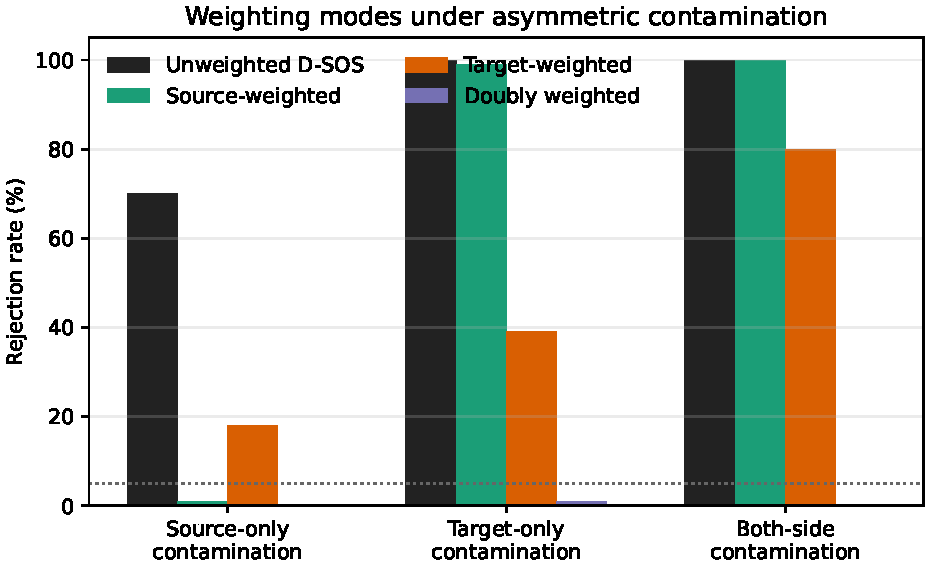
\includegraphics[width=0.95\linewidth]{figures/mode_comparison_plot.pdf}
	\caption{Asymmetric-diagnostic study. Contamination pattern (source-only, target-only, or two-sided) versus rejection rate. The dotted line marks the $5\%$ nominal level. Source-weighted and target-weighted diagnostics help only for one-sided contamination. The doubly weighted test remains calibrated when both sides contain irrelevant weak-overlap mass.}
	\label{fig:mode-comparison}
\end{figure}

\section{Second Synthetic Data-Generating Process}
\label{app:second-dgp}

The main text uses a univariate Gaussian overlap model. This appendix reports a second synthetic DGP with two-dimensional features and a linear score function. Source features are drawn from $\mathcal{N}(0, I_2)$. Target features are a mixture: $(1-\delta)$ fraction from $\mathcal{N}(0, I_2)$ and $\delta$ fraction from $\mathcal{N}((3,0), 0.5 \cdot I_2)$, where $\delta$ is the overlap-severity parameter. The severity score is $S = 0.5X_1 - 0.3X_2 + \epsilon$ with $\epsilon \sim \mathcal{N}(0, 0.5)$ for both groups, and harmful shift adds an intercept term to target scores on the common support. The domain classifier uses the first feature dimension only.

Figure~\ref{fig:second-dgp-calibration} confirms the calibration pattern: the doubly weighted test stays near nominal while unweighted testing over-rejects as overlap weakens. Figure~\ref{fig:second-dgp-power} shows power under harmful shift on the common support: the doubly weighted test responds to genuine harm while remaining calibrated at zero effect.

\begin{figure}[t]
	\centering
	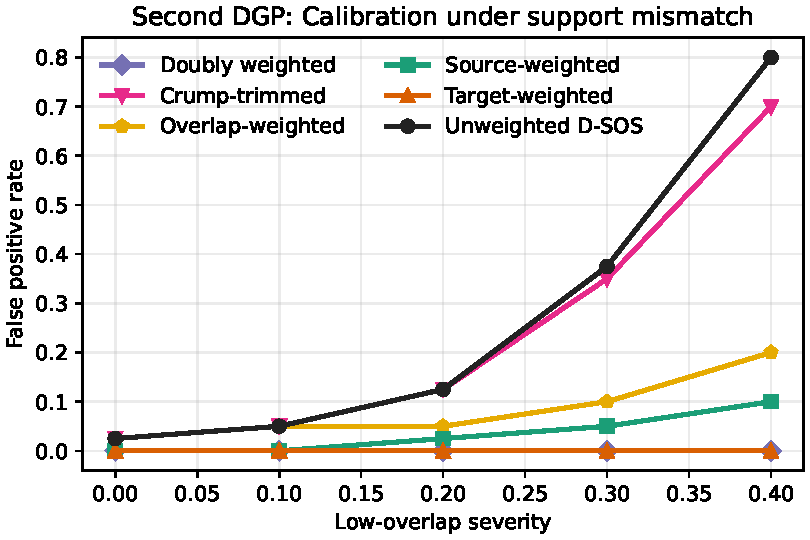
\includegraphics[width=0.95\linewidth]{figures/second_dgp_calibration_plot.pdf}
	\caption{Calibration under the second DGP. The doubly weighted test preserves calibration while unweighted and one-sided modes over-reject.}
	\label{fig:second-dgp-calibration}
\end{figure}

\begin{figure}[t]
	\centering
	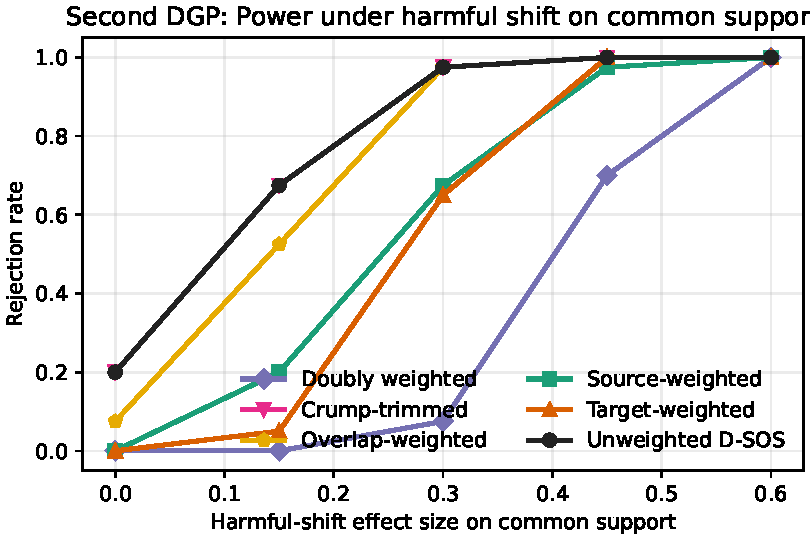
\includegraphics[width=0.95\linewidth]{figures/second_dgp_power_plot.pdf}
	\caption{Power under the second DGP. The doubly weighted test detects harmful shift on the common support while remaining specific at zero effect.}
	\label{fig:second-dgp-power}
\end{figure}

\section{Domain Classifier Sensitivity}
\label{app:domain-clf-sensitivity}

The main text uses logistic regression as the domain classifier. This appendix reports calibration under three classifier families: logistic regression, random forest ($100$ trees, max depth $5$), and histogram gradient boosting ($100$ iterations). The experiment replicates the calibration setup from the main text for each classifier.

Table~\ref{tab:domain-clf-sensitivity} reports the rejection rate of the doubly weighted test at each severity level. All three classifiers produce similar calibration: the doubly weighted test stays near the nominal $5\%$ level across the severity grid. The random forest and HistGBM produce more concentrated weights (lower ESS) because their flexible decision boundaries separate source and target more sharply, but this does not inflate false alarms.

\paragraph{Real-data classifier and split robustness.} The synthetic study isolates classifier choice; for the revision the HELOC checks will be repeated with an alternative domain classifier (random forest) and a perturbed split (ExternalRiskEstimate $>60$) to confirm the reported ESS and $p$-value regime. Committed \texttt{results/} and \texttt{figures/} were regenerated at the current protocol (9,999 permutation resamples, ten-fold domain-classifier CV); metadata hashes match the current tree (see Reproducibility Plan).

\begin{table}[t]
	\centering
	\caption{Doubly weighted rejection rate by domain classifier and severity (40 repeats, $\lambda = 0.5$).}
	\label{tab:domain-clf-sensitivity}
	\footnotesize
	\begin{tabular}{l c c c}
		\toprule
		Severity & Logistic & Random Forest & HistGBM \\
		\midrule
		0.0 & 0.00 & 0.00 & 0.00 \\
		0.1 & 0.00 & 0.00 & 0.00 \\
		0.2 & 0.00 & 0.00 & 0.00 \\
		0.3 & 0.00 & 0.03 & 0.00 \\
		0.4 & 0.00 & 0.00 & 0.03 \\
		\bottomrule
	\end{tabular}
\end{table}

\section{NSW Employment Experiment (Raw Outcome Score)}\label{app:nsw}

The National Supported Work (NSW) program~\cite{LaLonde_1986} contrasts experimental treated participants with an observational comparison group. We use the Dehejia--Wahba screened CPS comparison sample ($n=429$; evaluation $n=85$ after the source holdout) as source and the NSW treated group ($n=185$) as target, with post-program earnings in dollars as a continuous, higher-is-better severity score and no model-derived score (9,999 permutation resamples). Populations differ systematically in education, prior earnings, and demographics, creating feature overlap that mirrors weak-overlap settings from the synthetic experiments (doubly weighted ESS: $24$ of $85$ source, $57$ of $185$ target evaluation observations). The test does not reject under any mode (unweighted $p=0.131$, doubly weighted $p=0.508$; Crump-trimmed $p=0.660$, overlap-weighted $p=0.604$). Mean earnings are higher in the source ($\$7{,}832$) than in the target ($\$6{,}349$), yet no test flags the difference---contamination can mask harm as readily as it invents it. About a quarter of each group reports zero earnings, so ties are present but mild; the outcome is continuous dollars rather than a binarized threshold. The non-rejection should be read alongside the HELOC illustration in the introduction that contamination can both invent harm and hide it.


\end{document}
